\begin{figure}
\centering
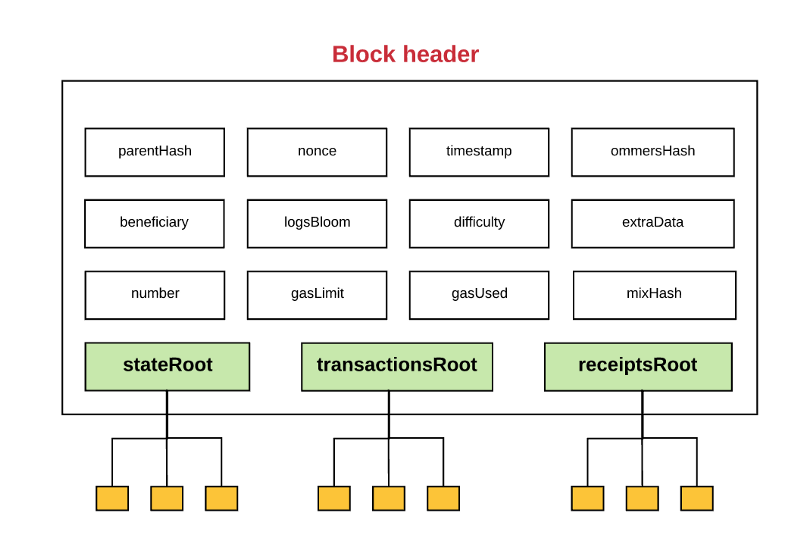
\includegraphics[width=0.55\textwidth, height=200px]{figures/block-headers.png}
\caption{Block headers \cite{preethi}}
\end{figure}

\begin{figure}
\centering
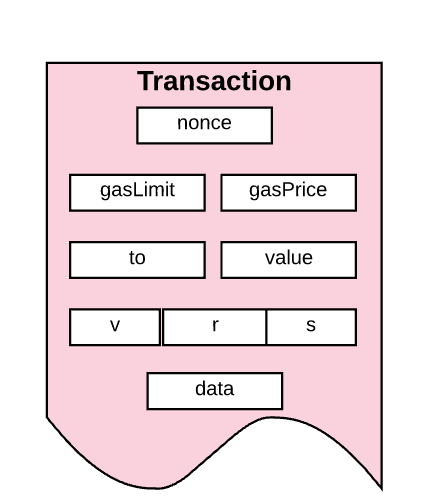
\includegraphics[width=0.45\textwidth, height=200px]{figures/transaction-contents.png}
\caption{Transaction contents \cite{preethi}}
\end{figure}

In order to access the data in any form of blockchain technology one must first be an owner of a full node of the respective network. 
This means that the whole blockchain data with all its records is stored on the researcher's device. 
However for the most part, data in this form is not stored in a manner that is easy to query. 
For this reason we opted to become owners of a full node of the Ethereum blockchain, to subsequently scrape the blockchain for the desired information and to store the results in a relational database, which in turn is easy to query.

The data-scraper is written in the \texttt{Python} language using the \texttt{web3.py} module \cite{Python, web3}.
Through \texttt{web3.py}'s interface it is possible to interact with the Ethereum blockchain. 
In particular the \texttt{web3.py} module enables us to extract information for every block and each transaction that is recorded in the blockchain.

\begin{algorithm}
\begin{algorithmic}
\State Check progress file if the ETL can be resumed from a block.
\If {yes}
    \State current block $c \gets$ content of progress file
\Else
    \State $c \gets 1$
\EndIf
\State $s \gets 2000000$ 
\While {$c \leq s$}
   \State Overwrite progress file with $c$ 
   \State $content_{Block} \gets \texttt{getBlock(c)}$
   \State $row_{Block} \gets \texttt{extractInfo(}content_{Block}\texttt{)}$
   \State $\texttt{write(} row_{Blocks}, \texttt{"Block")}$
   \For {each $transaction$ in $content_{Block}$}
       \State $row_{Transaction} \gets \texttt{extractInfo(}transaction\texttt{)}$
       \State $\texttt{write(} row_{Transaction}, \texttt{"Transactions")}$
   \EndFor
\EndWhile
\end{algorithmic}
\caption{Data Scraper: Overview}
\label{etl}
\end{algorithm}


\begin{figure*}
\centering
\begin{tikzpicture}[relation/.style={rectangle split, rectangle split parts=#1, rectangle split part align=base, draw, anchor=center, align=center, text height=3mm, text centered}]
% Relations

\node (usertitle) {\textbf{USERS}};

\node [relation=2, rectangle split horizontal, rectangle split part fill={lightgray!50}, anchor=north west, below=0.7cm of usertitle.west, anchor=west] (users)
{\underline{wallet\_address} \\ \texttt{VARCHAR}
\nodepart{two}   user\_id \\ \texttt{SERIAL}};

\node [below=1.3cm of users.west, anchor=west] (transactionstitle) {\textbf{TRANSACTIONS}};;

\node [relation=7, rectangle split horizontal, rectangle split part fill={lightgray!50}, below=0.7cm of transactionstitle.west, anchor=west] (transactions)
{block\_hash \\ \texttt{VARCHAR}
\nodepart{two}     value \\ \texttt{FLOAT}
\nodepart{three}   sender \\ \texttt{VARCHAR}
\nodepart{four}    receiver \\ \texttt{VARCHAR}
\nodepart{five}    gas\_used \\ \texttt{INT}
\nodepart{six}     gas\_price \\ \texttt{INT}
\nodepart{seven}   \underline{transaction\_hash} \\ \texttt{VARCHAR}};

\node [below=1.3cm of transactions.west, anchor=west] (blockstitle) {\textbf{BLOCKS}};

\node [relation=5, rectangle split horizontal, rectangle split part fill={lightgray!50}, below=0.7 cm of blockstitle.west, anchor=west] (blocks)
{block\_id \\ \texttt{SERIAL}
\nodepart{two}        \underline{block\_hash} \\ \texttt{VARCHAR}
\nodepart{three}      inception\_time \\ \texttt{INT}
\nodepart{four}       gas\_used \\ \texttt{INT}
\nodepart{five}       gas\_limit \\ \texttt{INT}};

% Foreign keys

\draw[-latex] (users.one south) --++ (0, -0.2) -| (transactions.three north);
\draw[-latex] (users.one south) --++ (0, -0.2) -| (transactions.four north);
\draw[-latex] (blocks.two north) --++ (0, 0.75) -| (transactions.one south);
\end{tikzpicture}
\caption{Database Model: the primary keys of each table are underlined, foreign keys are represented by arrows, the type of each column is capitalized.}
\label{datamodel}
\end{figure*}

In particular, for each block inside a predetermined range we query its contents and obtain the data that is interesting for the further analysis. 
On the block level we extract the hash of each block as a unique identifier and the time each block was inserted into the blockchain. 
Note that this is not necessarily the time that the transaction was being commissioned. 
Finally we query the total gas that was used for each block as well as the gas limit for each block. 
Along with that information we retrieve a list of transactions that are contained within that block.

Making use of the list of transactions within a block we extract the wallet addresses of both sender and receiver, as well as the total value, of the transaction. 
Additionally we retrieve information on the gas price for the transaction. 
Figure \ref{datamodel} summarizes the relations within that database and Algorithm \ref{etl} gives an outline of the datascraper in pseudocode.
